\chapter{Estado del Arte}\label{chapter:state-of-the-art}


\section{Tareas principales de los sistemas Generación de Lenguaje Natural}

    Hasta hoy considerado como el punto de referencia y texto más completo en el campo de GLN(\cite{Gatt2018SurveyOT}), el libro de Ehud Riter y
Robert Dale: Building Natural Language Generation Systems(~\cite{reiter_dale_2000}), sienta las bases y define las que se han asumido como tareas principales 
de un sistema de GLN:

\begin{itemize}
    \item Determinación del contenido: decidir qué información es relevante.
    \item Estructuración del texto: determinar en qué orden se presentará la información.
    \item Agregación: decidir qué información se presenta en cada oración.
    \item Lexicalización: encontrar las palabras y frases adecuadas para expresar información.
    \item Generación de expresiones de referencia: selección de las palabras y frases para identificar entidades del dominio.
    \item Realización lingüística: conformación del texto con oraciones bien formadas.
\end{itemize}

Cada una de estas tareas presenta un objetivo dentro del sistema y existen distintas técnias para su realización.
    
\subsection{Determinación del contenido}

    Cada sistema GLN tiene un objetivo comunicativo, lo cual hace necesario determinar que información del dominio es relevante y debe 
estar representada en el texto final(\cite{reiter_dale_2000}). Los sistemas pueden presentar una especificación de los datos de la entrada 
o seleccionar un subconunto de los mismos(\cite{reiter_dale_2000}).

    El reconocimiento de patrones es una de las t\'ecnicas utilizadas con este fin.  SumTime-Turbine(~\cite{Yu2006ChoosingTC}) es un sistema funcional para crear
 informes sobre un mecanismo de turbinas de gas. En un contexto donde la cantidad de datos en muy grande y en su mayoría irrelevante, 
 los autores con ayuda de los expertos del dominio crean un modelo que permite reconocer patrones en los datos así como luego, utilizando una base de datos de patrones 
antiguos determinar los patrones relevantes a ser expresados en el informe. 

    Existen muchos sistemas de GLN que utilizan modelos basados en reglas como \'unica metodolog\'ia para la selecci\'on de contenido(~\cite{reiter_dale_2000,Perera2017RecentAI}). Bouayad-Agha, Casamayor y 
Wanner (~\cite{BouayadAgha2011ContentSF}) en su trabajo presentaron el dise\~no te\'orico de un sistema para generar resumenes de partidos de 
futbol de la Liga Espa\~nola. Para la conformaci\'on del mismo describieron la construcci\'on de una garn base de conociminetos del dominio as\'i como 
un estricto sistema de reglas para la selecci\'on de contenido. Es relevante este enfoque ya que con un conocimiento del dominio a tratar y de la intenci\'on comunicativa del texto a producir 
es posible implementar reglas que den lugar a la selección del contenido relevante(~\cite{Reiter1997BuildingAN,reiter_dale_2000}). 

    Como el proceso de creaci\'on de reglas puede ser tedioso y es dependiente del dominio(~\cite{Reiter1997BuildingAN}) aparecieron iniciativas que para la automatizaci\'on de esta tarea. Un enfoque 
basado en t\'ecnicas de aprendizaje autom\'atico es el presentado por Dubou\'e y McKeown(~\cite{Dubou2003StatisticalAO}). En este trabajo plantearon un modelo de aprendizaje supervisado que a trav\'es de
un corpus de resultados deseados(texto escrito por humanos) aparejados con los tipos lingüísticos de la entrada(distintos tipos de datos que recibe el sistema) determina un conjunto de constantes. Estas constantes 
expresan si determinado dato de entrada debe aparecer o no reflejado en la salida y bajo que condiciones. Este sistema se utilizó para la generación de descripciones biográficos cortas que resumirán hechos 
importantes sobre personajes famosos.

\subsection{Estructuración del texto}

    La estructuración del texto o planificación del discurso es el proceso donde se da orden y estructura al conjunto de mensajes a expresar en el texto producido. En un texto la información se presenta en un orden particular 
y, por lo general, hay una estructura subyacente a la presentación. La complejidad de la estructura de los textos puede variar de un sistema a otro. Una buena estructuración puede hacer que un texto sea mucho más fácil 
de leer(~\cite{Reiter1997BuildingAN}).

    Los primeros enfoques para la estructuración de documento se basaron en reglas estructuradas hechas a mano dependientes del dominio(~\cite{Gatt2018SurveyOT}). A este enfoque se le conoce como el enfoque basado en esquemas, nombre que 
se deriv\'o del trabajo de Kathleen R. McKeown(~\cite{mckeown1985discourse}) cuando acu\~n\'o el t\'ermino \textit{"schematta"}. En la construcci\'on de su sitema TEXT(~\cite{mckeown1985discourse}), McKeown, luego del an\'alis de muchos 
ejemplos del dominio, concluyó que dado un objetivo comunicativo, la información tiende a transmitirse en el mismo orden. En base a esto defini\'o estructuras(esquemas) que determinan posibles combinaciones de atributos, formando patrones 
y plantillas. De esta forma el sistema, dada una intenci\'on comunicativa, puede seleccionar un esquema que defina la forma de transmitir la información. La mayor\'ia de los sitemas que siguen este enfoque utilizan 
las Matrices de Valores de Atributos(AVMs por sus siglas en inglés, Attribute Value Matrics)(~\cite{Perera2017RecentAI}).

    Las estructuras ret\'oicas son otro de los mecanismos que se utilizan para la planificación. Estas se derivan del trabajo de Mann y Thompson quienes introdujeron la Teor\'ia de la Estructura Ret\'orica(RST por
sus siglas en inglés, Rhetorical Structure Theory)(~\cite{mann1988rhetorical}). Las estructuras ret\'oricas constituyen un m\'etodo lingüístico para la descripci\'on de texto caracterizando las estructuras primarias del mismo y estableciendo 
relaciones funcionales entre sus distintas partes. La RST tiene como base los conceptos de n\'ucleo y sat\'elite que definen las partes del texto entre las que se estable un relaci\'on. Los distintos sistemas que utilizan las estructuras ret\'oricas 
para la estructuraci\'on del texto definen que tipo de relaciones establecen. Ejemplo de relaciones lingüísticas planteadas por Mann y Thompson en su trabajo son: motivaci\'on, causa, condici\'on, cirscuntancia, etc(~\cite{mann1988rhetorical}). 

\subsection{Agregación}

    En un texto, cada parte de información no tiene que estar presente en oraciones independientes. Hay escenarios donde es 
deseable que distintos mensajes sean transmitidos en una misma oraci\'on. La agreagaci\'on puede permitir crear texto de mayor 
calidad o eliminar repeticiones inncesarias que vayan en contra de la fluidez del texto(\cite{Gatt2018SurveyOT}).
    Un ejemplo de agregaci\'on, en el dominio del f\'utbol, describiendo el hecho de dos anotaciones consecutivas de un jugador, puediera ser:

\begin{itemize}
    \item (1) Ronaldo anot\'o para el Real Madrid en el minuto 2. Ronaldo anot\'o para el Real Madrid en el minuto 8.
    \item (2) Ronaldo anot\'o dos veces para el Real Madrid antes del minuto 8.
\end{itemize}

    En (2) se evita la repetici\'on y la información se presenta de forma m\'as fluida y natural al lector.
    
    Reape y Mellish(~\cite{reape1999just}) realizaron un estudio sobre la tarea de agregación dentro de los sitemas de generación 
de texto, distinguiendo entre la agregación a nivel semántico(más dependiente del dominio) y a nivel sintáctico. Muchos de los primeros 
trabajos sobre agregación fueron dependientes del dominio, centrados en la aplicación de reglas(por ejemplo, 
"si un jugador marca dos goles consecutivos, expr\'esalo en la misma frase') generalmente hechas a mano(ejemplo ~\cite{Shaw1998ClauseAU}). 
Con el tiempo aparecieron propuestas que utilizan enfoques de aprendizaje autom\'atico. SPoT es un sistema que se present\'o en ~\cite{walker2001spot}) 
contituendo uno de los primeros sistemas entrenados que incluye la tarea de agregación. Los autores plantearon una metodolog\'ia basada en la producci\'on 
de varios textos para una misma entidad informativa utilizando diferentes cl\'ausulas de agregación asociadas al dominio. Despu\'es utilizaron un modelo 
entrenado para dar un valor a cada una de las salidas estableciendo un ranking a partir del cual hacer la selección. Mientras, Barzilay y Lapata(~\cite{Barzilay2006AggregationVS})
plantearon el problema en términos de optimización global. Realizan una clasificación inicial sobre pares de entradas de la base de datos que determina 
si deben agregarse o no en función de su similitud por pares. Posteriormente, seleccionan un conjunto globalmente óptimo de entradas relacionadas en función
de un grupo de restricciones.

    Con la agregación sintáctica, podría decirse que es más factible definir reglas independientes del dominio para eliminar la 
redundancia(~\cite{Gatt2018SurveyOT}). Por ejemplo, convertir (3) en (4) a continuación

\begin{itemize}
    \item (3) Ronaldo marcó en el minuto 2 y marcó de nuevo en el minuto 8.
    \item (4) Ronaldo marcó en el minuto 2 y de nuevo en el 8.
\end{itemize}
    
podría lograrse identificando las frases verbales paralelas en las dos oraciones conjuntas y eliminando el sujeto y el verbo en la segunda.

\subsection{Lexicalización}

    La lexicalización es un proceso muy importante dentro de un sitema de GLN. Es el proceso durante el cual se 
seleccionan la palabra o palabras que expresan un concepto o relaci\'on(~\cite{Reiter1997BuildingAN}). Una de las 
complicaciones del proceso de lexicalización est\'a dada porque una misma relación puede ser expresada de 
distintas formas. Por ejemplo, el evento de la anotación de un gol en un partido de fútbol puede ser expresado como:
¨marcar un gol¨, ¨poner el balón en la red¨, ¨conseguir una anotación¨. La complejidad de este proceso depende en gran 
medida del número de alternativas que el sistema pueda o quiera contemplar. Las restricciones contextuales también juegan 
un papel importante a la hora de expresar un mensaje, por ejemplo, la expresion ¨marcó un gol¨ es desafortunada si el evento 
descrito es un gol en propia puerta(~\cite{Gatt2018SurveyOT}).

    El proceoso de lexicalización puede seguir dos vertientes principales. Una ser\'ia la realizaci\'on de la  
lexicalización de la forma m\'as simple posible, lo cual se lleva a cabo generalemente utilizando t\'ecnicas para el llenado de 
plantillas lexicalizadas. De otra forma se puede realizar este proceso en mayor profundidad utilizando t\'ecnicas m\'as complejas  
que permmitan por ejemplo: la eliminaci\'on de palabras innecesarias, la selección de vacablos que maximicen la efectividad del obetivo 
comunicativo del texto, la uni\'on de t\'erminos que se aparejan frecuentemente en el dominio(~\cite{Perera2017RecentAI}).

    Los enfoques basados en reglas son de los m\'as utilizados, pudiedo variar en complejidad entre un sistema y otro. \textit{EasyText}(~\cite{danlos2011easytext}) 
es un ejemplo de sistema que utiliza reglas para la lexicalización pero que da un paso m\'as all\'a ya que consume de una base de datos 
l\'exica creada principalmente por lingüístas. Esta alternativa permite una lexicalización m\'as avanzada pero a su vez es altamente 
costosa en recursos.

    La utilizaci\'on de ontolog\'ias tambi\'en est\'a presente en este proceso de los sistemas de GLN. El uso de ontologías permite 
al sistema ganar en adaptabilidad ya que encontrar una ontología para un dominio determinado es más sencillo que encontrar un corpues para 
el mismo. Así mismo ofrecen una mayor cobertura de las representaciones semánticas que los corpus(~\cite{Perera2017RecentAI}). En ~\cite{cimiano2013exploiting} introducen 
un modelo que utiliza este enfoque presentado en el dominio de las recetas de cocina.


\subsection{Expresiones de referencia}

    Robert Dale y Ehud Rither describieron la generación de expresiones de referencias dentro de un sitema de GLN como la tarea de 
indentificar la expresión, comprensible de cara al usuario, a utilizar para indetificar a una instancia del dominio(~\cite{reiter_dale_2000,Gatt2018SurveyOT}). 
Los primeros m\'etodos para la selección de referencias fueron los algoritmos generativos que en común presentan la necesidad de tener conocimiento 
contextual y de propiedades de las entidades(~\cite{Gatt2018SurveyOT}). De este orden es el algoritmo incremental cuya base se plant\'o en ~\cite{dale1995computational}. 
El algoritmo, en base a conocer la entidad a referenciar(objetivo), el resto de entidades(llamadas distractores) y el grupo de propiedades que definen entidandes en el dominio,
busca determinar un conjunto de propiedades \'unicas que definan al objetivo y lo diferencien del resto.

    Muchos de los trabajos que versan sobre este tema hacen énfasis en un tipo determinado de referencia(~\cite{ferreira2018neuralreg}). La selección 
puede ser de un pronombre(\'el/ella), una descripci\'on( Sim\'on, el jugador cubano) o en la generación de nombres propios(Frederich Cepeda/Cepeda). 
Rither y Dale(~\cite{reiter_dale_2000}) plantean una diferencia entre una referencia temprana(primera vez que se menciona una 
entidad en el texto) y una tard\'ia(cuando se refiera a una entidad mencionada anteriormente). Plantearon el uso de los nombres propios a la hora 
de introducir una entidad, luego, en base a cla\'usulas seleccionar un pronombre apropiado, ejemplo:

\begin{verbatim}
    si el referente fue mencionado en la oración anterior;
    entonces utiliza un pronombre
\end{verbatim}

a su vez es necesario considerar los escenarios donde la generaci\'on de expresiones de referencia pudiera llevar a ambigüedades:

\begin{itemize}
    \item Benzema anotó dos para el Real Madrid mientras Luka Modric brindó dos asistencias. Él fue elegido el jugador del partido... 
\end{itemize}

    En \cite{siddharthan2011information} los autores realizaron un estudio emp\'irico del comportamiento de las referencias hacia parsonas basadas en 
su nombre propio en el contexto de los art\'iculos de noticias. Para ello utilizaron un corpus de noticias en inglés de diferentes agencias de prensa y 
cuantificaron las diferentes formas de referencia seg\'un el momento referencial de la instancia(temprana o tard\'ia). Como resultado de este trabajo 
arrojaron que el nombre completo de la entidad suele utilizarse como primera referencia en la pr\'actica totalidad de los casos mientras que en su mayor\'ia
el apellido se utiliza cuando se trata de una referencia tard\'ia. 

   %Entre las propuestas recientes para la generaci\'on de entidades referenciales encontramos la presentada en \cite{ferreira2018neuralreg}. Los autores presentan 
%\textit{NeuralREG}, un modelo de aprendizaje profundo implementado como multi-encoder, attention-decoder con biderectional LSTM(Long-Short Term Memory). Para el 
%entrenamiento del modelo utilizaron una versi\'on deslexicalizada del corpus \textit{WebNLG} . Cada entidad presente en los datos fue mapeada
% con diferentes etiquetas de forma tal que 

\subsection{Realización lingüística}

    El proceso de realizaci\'on lingüística es el que da lugar a la formaci\'on final del texto expresado en oraciones con una 
estructura gramatical correcta y coherente con el mensaje a transmitir. Esta tarea implica ordenar los constituyentes de una oración, 
así como generar las formas morfológicas correctas (incluidas las conjugaciones y la concordancia de los verbos). A menudo, los 
realizadores también necesitan insertar palabras funcionales (como verbos auxiliares y preposiciones) y signos de puntuación(~\cite{Gatt2018SurveyOT}).
   
    Una de las t\'ecnicas m\'as utilizadas es la que incluye el uso de plantillas predefinidas para expresar mensajes(\cite{Gatt2018SurveyOT}). Las 
plantillas, aunque requieren una carga intensiva de trabajo para lograr mayor variabilidad en el texto a producir permiten un control total sobre 
la calidad y la correctitud del texto a elaborar. Un ejemplo de plantilla:

\begin{verbatim}
    $equipo_1 venció $pts_equipo_1 a $pts_equipo_2 a $equipo_2
\end{verbatim}

    Dicha plantilla, que representa el resultado de un enfrentamiento entre dos equipos se completa con la información extraida de los datos y a la hora de 
la realización el resultado pudiera ser el siguiente:

\begin{verbatim}
    Industriales venció 10 a 1 a Granma
\end{verbatim}

\section{Propuestas neuronales para la generación de texto}
    Al ingual que en otras áreas del procesamiento de lenguaje natural, el dominio de la GLN se ha visto 
impactado por el auge de las soluciones basadas en redes neuronales (~\cite{Gatt2018SurveyOT,sharma2022innovations}). 
Mientras los sistemas tradicionales de D2T siguen una estructura modular con etapas bien definidas (estructuración, relalización, etc), 
los modelos neuronales variaron el camino hacia estructuaras \emph{end-to-end} (de extremo a extremo, en español), unificando 
en muchas casos, varias tareas en un solo paso de entrenamiento.

    Los trabajos que siguieron este enfoque (~\cite{lebret-etal-2016-neural,mei2016talk,wiseman-etal-2017-challenges} ) plantearon modelos \emph{Seq2Seq} (de secuencia a secuencia, en español) que adoptan la 
influyente estructura de codificador-decodificador (~\cite{sutskever2014sequence}). Utilizan una red neuronal recurrente (RNN, \emph{Recurrent Neural Network}, en inglés) 
para codificar la entrada de un vector de representación el cual sirve a su vez como entrada auxiliar de otra RNN que hace de decodificador y produce el texto, y no tienen módulos 
específicos para mejorar la calidad del resultado más allá de los mecanismos gen\'ericos de atención y copia (~\cite{bahdanau2014neural,gu2016incorporating}). La popularidad de los módelos 
\emph{end-to-end} se vió impulsada y a la vez creó la necesidad de contar con corpus de datos paralelos que permitieran evaluar la calidad de las propuestas. Estos conjuntos de datos tenían que 
tener la suficiente cantidad de instancias para poder entrenar modelos de estas características. RotoWire (~\cite{wiseman-etal-2017-challenges}) es un punto de referencia ampliamente utilizado, se construyó con cerca de 
cinco mil pares de datos estadísticos de partidos de baloncesto y su correspondiente resumen descriptivo escrito por profesionales. En ~\cite{puduppully2019data}, los autores introdujeron MLB, un nuevo corpus con aproximadamente 
25 mil instancias de estádisticas aparejadas con descripciones en este caso en el dominio del beisbol. Otros conjuntos de datos hechos a mano como E2E (~\cite{novikova2017e2e}) se han construido para analizar tareas espec\'ificas 
como la capacidad de realización lingüística.

        \begin{figure}[!]
            \begin{center}
                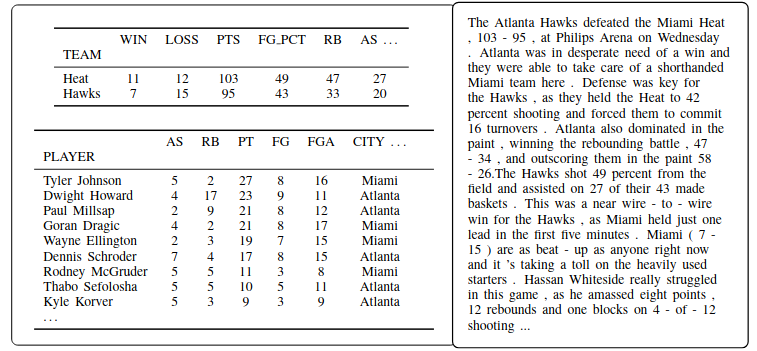
\includegraphics[width=\textwidth]{Graphics/rotowire_instancia.png}
            \end{center}
            \caption{Instancia de RotoWire (~\cite{wiseman-etal-2017-challenges}).}
            \label{fig_RotoWire}
        \end{figure}

 En ~\cite{wiseman-etal-2017-challenges} los autores mostraron la capacidad de estos modelos de producir un texto dotado de mayor 
fluidez en comparativa con propuestas tradicionales. A su vez, además de ser propensos a la alucinación (es decir, generan texto que no es compatible con la entrada), 
mostraron  deficiencias a la hora de seleccionar el contenido y/o estructurar el documento (por ejemplo, en el marco de una descripción biográfica, la omisión de la fecha de nacimiento es un relevante, 
mientras que de aparecer no es apropiado que lo haga en la última oración del escrito ). Para mejorar esta situación ~\cite{puduppully2019dataselandplan}  
presentaron una arquitectura que incorpora selección y planificación de contenido sin sacrificar el entrenamiento \emph{end-to-end}. Descompusieron la tarea de generación en dos etapas. Dado el corpus de 
registros de datos (junto con las descripciones), primero generaron un plan de contenido destacando qué información debía mencionarse y en qué orden para luego generar el documento teniendo en 
cuenta dicho plan. Un enfoque similar se planteó en ~\cite{chen2021neural}, mientras que en ~\cite{moryossef2019step}, desacoplaron por completo ambas fases, dejando solo el modelo neuronal para la realización del 
texto una vez desarrollada la estructura informativa.

        \begin{figure}[!]
            \begin{center}
                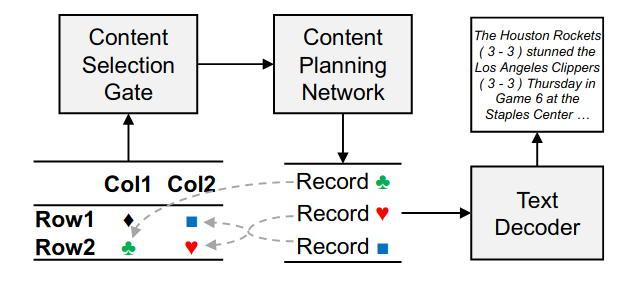
\includegraphics[scale=0.4]{Graphics/lapata_arquitectura.png}
            \end{center}
            \caption{Arquitectura del modelo presentado en ~\cite{puduppully2019dataselandplan}.}
            \label{fig_lapata_arquitectura}
        \end{figure}


    La utilización de modelos preentrenados en tareas de generación de texto-a-texto para producir texto a partir de datos en base al reentrenamiento 
fue de los enfoques que se exploraron recientemente. En (~\cite{kale2020text}) los autores utilizaron el modelo T5 (\emph{“Text-to-Text Transfer Transformer”}, su nombre en inglés) (~\cite{raffel2020exploring})
preentrenado para tareas de generación de resúmenes, traducción entre idiomas, clasificación de texto entre otras. Sus resultados fueron alentadores sobre todo desde el punto de vista de 
la generalizción. Este modelo, no solo tuvo una buena actuación en cuanto a la calidad del texto generado sino que también mostró buena adaptación a dominios distinos a los 
del reentrenamiento, lo cual constituyó una diferencia respecto a los modelos neuronales tratados anterioremente.


    Como quedó patente en (~\cite{wiseman-etal-2017-challenges,ferreira2019neural,duvsek2020evaluating,sharma2022innovations})  los sitemas basados en redes neuronales
 son capaces de producir texto que supera en fluidez y en evaluaciones humanas como la naturalidad a los sistemas tradicionales. Por contra, 
estos modelos siguen lidiando con su principal problema que es la presencia de alucinacinaciones en las salidas. Esta deficiencia es objeto de interés 
de los investigadores en este campo (~\cite{ji2022survey}). Por esta razón, Robert Dale, en su \textit{Natural language generation: The commercial state of
the art in 2020} (~\cite{dale2020natural}) planteó que estas soluciones, aunque prometedoras, se 
encuentran en fase principalmente académica y que en la industrian, en un entorno donde la fidelidad de los datos es crucial, su adopción general no ha llegado.   


\section{Sistemas para la generación de texto a partir de datos}

    Al referirse al campo de GLN, se puede afirmar que el mismo es ya un campo investigativo consolidado dada la cantidad 
de sistemas que han sido implementados y la variedad de los dominios de su aplicación práctica. FOG (\emph{Forecasting Generator}, en inglés) (~\cite{goldberg1994using}) es 
de los primeros sistemas funcionales para la generación de texto a partir de datos. Este, al igual que SumTime (~\cite{reiter2005choosing}) genera breves pronósticos del tiempo
a partir de los valores de variables meteórologicas. 

    En la escena industrial, propiciado por el desarrollo constante de herramientas para el análsis y captura de datos,
hubo empresas que detectaron en la generación de texto un nicho de mercado no cubierto y prometedor (~\cite{dale2020natural}). Compañías como \textit{Ax Semantic\footnote[1]{https://en.ax-semantics.com/}} y 
\textit{Narrativa\footnote[2]{https://www.narrativa.com/}} ofrecen soluciones para automatizar la descripción de productos para el comercio electrónico. 
\textit{Automated Insights} creó su plataforma para la generación de lenguaje natural, \textit{Wordsmith}. Este software da la posibilidad al usuario de crear un conjunto 
de plantillas basadas en reglas que desciben los datos que desea a tratar. A partir de las mismas, y en dependencia de su sofistición los textos generados pueden llegar a ser 
indistinguibles de los textos redactados por un humano. Precisamente en colaboración con \textit{Automated Insights}, la gran corporación de prensa \textit{Associated Press (AP)} generó l
las vistas previas de los partidos de una temporada regular de baloncesto, liberando a los periodistas de este trabajo. A su vez, \textit{Yahoo!} utiliza esta tecnología para crear informes 
de jugadores y resúmenes de partidos de fútbol del juego \textit{Fotball Manager} que es de gran interés para sus usuarios. Otro caso de uso dentro de la automatización de contenido en la prensa lo encontramos en \textit{PostData\footnote[3]{http://www.postdata.club/index.html}}, un sitio de periodismo 
de datos cubano, donde utilizan un modelo propio, \textit{ArmandBot} (~\cite{balboa2020}), para generar reportes sobre las actuaciones de los peloteros cubanos en grandes ligas.

    En la literatura hay propuestos varios modelos de sitemas para la GLN en el ámbito del deporte. Por ejemplo, en (~\cite{kanerva2019template}), apoyados en la constucción de un corpues de 2000 encuentros de hockey sobre hielo 
proponen un modelos de secuencia a secuencia, para generan narrativas sobre esta práctica deportiva. Hasan (~\cite{hasan2011automatic}) propuso un sistema basado en plantillas que sigue la arquitectura tradicional basada en módulos para 
modular para generar texto en inglés y bengalí\footnote[5]{El bengalí es el idioma nacional y el idioma oficial de la República Popular de Bangladesh} para generar resúmenes de juegos de críquet a partir de datos estructurados obtenidos de la web. 
Siguiendo el mismo enfoque, en ~\cite{gu2016incorporating} presentan otro sistema basado en plantillas para el críquet, en este caso al estilo propio de Sri Lanka.
 
En el caso del fútbol, una de las principales propuestas fue GoalGetter (~\cite{theune2001data}), un sistema de datos a voz en idioma neerlandés, que consta de dos módulos, uno para tranformar los datos en texto y 
otro para luego llevar el texto a sonido. GoalGetter tomó los datos de una página de Telexto que contenía los datos de uno o más partidos de fútbol. Una característica de este sistema es que propuso una arquitectura diferente al 
estándar modular de otros sistemas. En este caso, utilizó un solo módulo para la generación de texto que consumía una base de conocimiento con los nombres de los jugadores y equipos junto a un sistema de plantillas sintácticas.
 En base a este trabajo, en \cite{aires2016automatic} se propuso GameRecapper, un sistema capaz de generar resúmenes de partidos de fútbol de la liga portuguesa en idioma portugés. Este sistema obtenía los datos de \textit{www.zerozero.pt} 
una página web que contenía la información de partidos los partidos de cada jornada. Al módulo de generación agregaron a su vez una base de conocimiento y un conjunto de funciones léxico semánticas para mejorar la calidad del texto. De este trabajo es resaltó el hecho 
de que hicieron una caracterización más amplia del evento principal del fútbol, el gol, en su sistema de plantillas. Para cada distinto escenario propusieron la creación de plantillas oracionales específicas (primer gol del patido, último gol, gol que empata, etc).
Pass (~\cite{van2017pass}), es una propuesta basada en GoalGetter que busca diferenciar el texto producido en base a la audiencia del mismo. Para ellos establecen un sistemas de plantillas que abarca distintos posibles escenarios de resultado de un partido: victoria o derrota 
del equipo local, victoria o derrota del equipo visitante o empate. La elección de cual plantilla utilizar va en depencia de a qué afición irá dirigido el texto.  

    La gran mayoría de estos sistemas cuentan con un dominio específicos de aplicación, así como cuentan con una fuente de datos de la 
cual extraer la información a desarrollar. Por tanto, y aunque fuera posible la adaptabilidad, existe una depencia de la fuente de información. A su vez, el tener un dominio bien definido  
permite agreagar bases de conocimiento previo del mismo que enriquezcan los modelos. Predominan los sistemas basados en plantillas y reglas, variendo entre si su nivel de complejidad. Estos 
sistemas son especialmente adaptables y prácticos para idiomas distintos del inglés debido a que las herramientas de generación específicas desarrolladas son menores en compaaración (~\cite{gunasiri2021automated}). 
    En el presente trabajo se presenta un prototipo de sistema basado en la propuesta de un esquema general que permita definir esquemas específicos de entradas en formas de 4-tuplas (tuplas de cuatro elementos) de 
conocimiento de un deporte de enfrentamiento dos a dos ( beisbol, voleibol, judo, etc). A su vez, se seleccionan dos deportes, en este caso, futbol y boxeo, y a partir de las especifiaciones planteadas se 
se definen dos modelos capaces de generar un resumen informativo del evento en cuestión. Los modelos siguen el estandar basado en reglas plantillas simples de expresiones y oraciones.
    
    %\begin{figure}[htbp]
    %    \begin{center}
    %        %\includesvg{Graphics/arquitecturatesis3.svg}
    %        \includegraphics[width=\textwidth]{Graphics/arquitecturatesis3.svg}
    %    \end{center}
    %    \caption{Arquitectura del modelo propuesto}
    %    \label{arquitecturadelmodelo}
    %\end{figure}


